\section{Data Review}

    \subsection{NAO Data}

        Information about the state of the North Atlantic Oscillation, both daily and monthly, as used in this project, is available through the National Oceanic and Atmospheric Administration (NOAA) web portal. The calculation basis for the index is based on \cite{ClassificationSeasonalityandPersistenceofLowFrequencyAtmosphericCirculationPatterns}, employing Rotated Principal Component Analysis (RPCA) on monthly standardised 500-mb height anomalies from the CDAS within $20^\circ$N to $90^\circ$N from 1950 to 2000. The anomalies are determined by comparing the daily mean and standard deviation of the climatological average of 1950-2000 with the current values.
        
    \subsection{Storm Track Data}
    \label{sec:stormtrackdata}

        The foundation of this project are storm tracks provided by Hodges K. (2023). These tracks are primarily sourced from the European Centre for Medium-Range Weather Forecasts (ECMWF) reanalysis project, ERA5 \citep{ERA5globalreanalysishttps://doi.org/10.1002/qj.3803}. They were generated by a tracking algorithm designed to identify and follow points of relative vorticity at 850~hPa as outlined in \cite{NewPerspectivesontheNorthernHemisphereWinterStormTracks}, \cite{AdaptiveConstraintsforFeatureTracking}, and \cite{FeatureTrackingontheUnitSphere}. The tracks cover a period from 1940 to 2022 and have higher spatial resolution than tracks generated through older ERA projects, with the new tracks making use of T63 versus older projects based on T42, resulting in a decrease in grid cell spacing from roughly $2.8^\circ$ to $1.9^\circ$. The temporal resolution has also been increased from 3 to 1 hour.
        
        The tracks contain hourly data on the points of greatest relative vorticity, lowest mean sea-level air pressure, highest wind speed recorded around the storm at 925~hPa and highest wind speed recorded around the storm at 10m above the surface along with the relevant position in latitude and longitude for each of the listed data points.

        In this project, we also make use of the Extreme Wind Storms (XWS) catalogue \citep{XWS-nhess-14-2487-2014}. A publicly available catalogue containing information on European windstorms, covering 1979 to 2012, and consists of severe events that have caused high (re)insurance loss or have associated with them a high Storm Severity Index (SSI). SSI is calculated as a function of the storm area and maximum 925~hPa wind speed.
        
    \subsection{Wind Data}

        ERA5-Land, developed by \cite{munoz2019era5land} and the ECMWF, is an improvement on the ERA5 dataset and focuses exclusively on variables over land, spanning the period 1950 to 2023. It makes use of a finer grid spacing than ERA5, $0.1^\circ$ by $0.1^\circ$ ($\approx 9 \times 9 $km) compared to $0.25^\circ$ by $0.25^\circ$ ($\approx 23 \times 23 $km). The lapse rate has been adjusted to account for this higher spatial resolution and integrates ERA5 atmospheric variables as atmospheric forcing.

        ERA5-Land data are organised as follows: Each dataset comprises numerous data points distributed across a geographic grid. Consider each point as a representation of wind speed, orientated either North or East. These points are organised within a matrix, where rows and columns correspond to latitude and longitude, respectively. Thus, by identifying a point's position within the matrix, we can deduce its geographical coordinates. The dimensions of this matrix reflect our designated study area, and each matrix pertains to a specific moment, such as 14:00 on 01 Jan 1990. For every timestamp, two matrices are available: one for Northward wind measurements and another for Eastward ones. Together, these matrices allow us to determine both the magnitude and direction of the wind. These matrices are updated every hour, and the spacing between individual points in a matrix is 0.1 degrees.

\section{The New SSI Method}

    For the purposes of this study, a new method is developed to estimate the destructiveness of windstorms. It does this based on the energy carried by the wind near the surface, which is calculated by modifying the classic Kinetic Energy equation (Equation \ref{eq:KEfundamental}) and the equation for Mass Flow Rate (Equation \ref{eq:MassFlowRate}).
    
    \begin{equation}
    \label{eq:KEfundamental}
        \mathbf{KE} = \frac{1}{2} m\mathbf{v}^2
    \end{equation}

    \begin{equation}
    \label{eq:MassFlowRate}
        \dot{m} = \rho \mathbf{v} \cdot \mathbf{A}
    \end{equation}

    Where $\mathbf{KE}$ is the Kinetic Energy in the direction of the velocity vector, $m$ is the mass of the object, and $\mathbf{v}$ is the velocity vector taken to be the speed and direction of the wind at 10 m. $\dot{m}$ is the change in mass with respect to time of a fluid, $\rho$ is the density of the fluid and in this study is set to a constant value of $\rho = \rho_{air}\, \left(20^{\circ}C,\: 1024hPa\right) \approx 1.2$ kg/m$^3$. $\mathbf{A}$ is the cross-sectional vector area, with its surface orthogonal and its direction perpendicular to the velocity vector (Figure \ref{fig:volumeflowrate}). $\mathbf{A}$ has a fixed height of 10m, while its width is a function of wind direction, latitude, and longitude. The complete methodology for calculating $\mathbf{A}$ is presented in Section~\ref{sec:Calculating the cross-sectional vector area}. 

    \sidecaptionvpos{figure}{t}
    \begin{SCfigure}
        \centering
        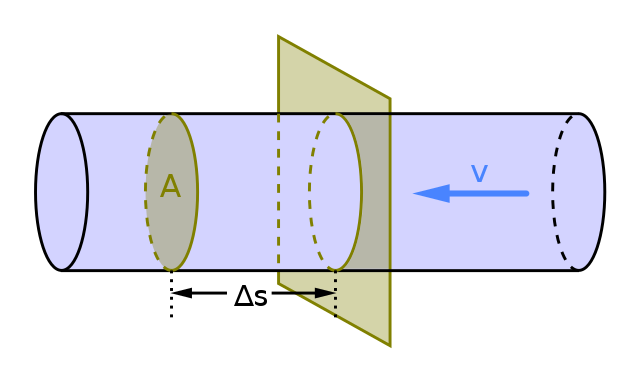
\includegraphics[width=0.6\textwidth]{figures/640px-Volumetric-flow-rate.svg.png}
        \caption{Visualisation of mass flow rate, with $\mathbf{v}$ the velocity vector and $\mathbf{A}$ the cross-sectional vector area. Adapted from MikeRun via Wikimedia Commons under license CC BY-SA 4.0. $\Delta \mathbf{s}$ is related to the volume flow rate and can be ignored.}
        \label{fig:volumeflowrate}
    \end{SCfigure}
    
    To combine Equation \ref{eq:KEfundamental} and Equation \ref{eq:MassFlowRate} we express the mass $m$ through the mass flow rate $\dot{m}$. The first step is to separate variables for the derivative $\mathrm{d}m/\mathrm{d}t$, and then integrate, which transforms Equation \ref{eq:MassFlowRateIntegrating} into Equation \ref{eq:MassFlowRateIntegrated}.
    
    \begin{equation}
    \label{eq:MassFlowRateIntegrating}
        \int \mathrm{d}m = \int \rho \mathbf{v} \cdot \mathbf{A} \mathrm{d}t
    \end{equation}

    \begin{equation}
    \label{eq:MassFlowRateIntegrated}
        m = \rho \mathbf{v} \cdot \mathbf{A} t
    \end{equation}

    By substituting Equation \ref{eq:MassFlowRateIntegrated} into Equation \ref{eq:KEfundamental} (referenced as Equation \ref{eq:KEandMassFlow}), we derive Equation \ref{eq:KE}. This gives us the Kinetic Energy, in Joules, of the wind at 10m.

    \begin{equation}
    \label{eq:KEandMassFlow}
        KE = \frac{1}{2} \left(\rho \mathbf{v} \cdot \mathbf{A} t \right) \mathbf{v}^2
    \end{equation}

    \begin{equation}
    \label{eq:KE}
        KE = \frac{1}{2} \rho \mathbf{v}^3 \cdot \mathbf{A} t
    \end{equation}

    Applying Equation \ref{eq:KE} to a data grid in an area of interest allows us to study the strength of a storm in its entirety or focus on a particular location. It also provides a robust way of ranking long-lasting storms of moderate intensity against short-lived and violent events.

    To the best knowledge of the author, this method appears novel within the field; however, there are examples \citep{web:psuWindEnergy} where the underlying equation is used in estimating the energy supplied to wind turbines by taking a derivative with respect to time of Equation \ref{eq:KE} which provides the wind power in watts.
    
    \subsection{Rationale for Development}

        The primary purpose of developing the energy method is the need for a method which recognises the irregular structure of a windstorm. Winds inside a windstorm can vary in speed depending on topography, pressure gradients, temperature differences, etc. which means that storms with similar parameters such as maximum vorticity or highest wind gust can vary in destructiveness. Another problem the energy method addresses is the difference between storms that are destructive not because of the severity of their winds, but because of their size and duration, where the loss accumulates and can become just as costly as a more violent event.

        It is of increased complexity compared to more common methods and requires the execution of code, including when obtaining an SSI for a singular storm/event. It is based off of wind data over the area of interest, and its performance is proportional to the resolution of the data, both in space and in time. 
        
\section{Analysis of Wind Energy in Storms}
    \subsection{Finding a Windstorm}

        The first step to analysing windstorms is knowing when and where a windstorm is. In this section, we go over the method used to sieve through storm track data (see Section \ref{sec:stormtrackdata} for more information on storm tracks) in order to compile a list of relevant windstorms and their start and end dates. The first step is to narrow the storm tracks to only those within our area of interest - western Europe, excluding Iceland ($\phi \in (42^\circ \rightarrow 72^\circ$\textbf{N}), $\lambda \in (-12^\circ \rightarrow 32^\circ$\textbf{E})).

        Since not all storm tracks develop into windstorms, we also apply a wind speed threshold that excludes data points that have a wind speed below 20~m/s at 10m. While there is not a consensus on the exact wind speed which defines a windstorm, we can estimate a range by observing past windstorm events and through the Beufort wind strength scale. Beufort 8 wind speeds, starting at 17~m/s, mark the point after which the wind becomes destructive to the environment. For Beufort 8, this manifests itself in the form of twigs and branches snapping off of trees. In this study, we will consider 17~m/s to be the minimum border for winds that can be considered part of a windstorm. The windstorm with the lowest maximum wind speed in the XWS Catalogue is windstorm Emma with 25~m/s at 925hPa over land. Thus 25~m/s is most likely the maximum threshold we can set without being overly exclusive. 20~m/s was selected through trial as the value within this range that best captures the storms listed in the XWS Catalogue.
        
        % As the track data were global and not limited to a particular location, a rough filter was applied, which excluded any data outside of a region of interest defined to be within 72 to 42 North and 12 West to 32 East. The resulting list of tracks contained noise in the form of tracks that did not develop into a storm. The reason for this is that when following a storm track, a point of low pressure and high vorticity is identified and followed over time, with wind speed measured in a fixed radius around the centre of the storm, but the method does not discriminate for the wind speed itself. To address this, another filter was added that removed all datapoints with wind speed below a certain threshold, in this study set at 20~m/s. This is a high threshold as windstorms are considered to be destructive at 17~m/s which coincides with the lower end of Beufort 8 winds, the point at which twigs begin to break off of trees, and slight structural damage can occur.
        
        Before further filtering was applied the result of implementing a minimum wind threshold resulted in a significant ammount of data points positioned over water, however, we are interested in windstorms over land as that is where they are most impactful. Due to the higher thermal conductivity of water and the lack of topographical obstacles, many storms in the dataset had their lifetime maximum over the water. Even storms that had a centre over land (determined by the point of highest vorticity) would continue displaying their wind speed over the ocean and as such it is challenging to estimate their destructiveness on land. To overcome this issue, we create a filter which removes all data points of storms with a centre above water and a wind speed below the threshold. The remaining fractions of storm tracks have a high potential of belonging to European windstorms. The reason we say that they are fractions of storm tracks is that as a storm centre moves on and off land, due to the removal of all points over water, gaps in the track appear. To fix this patch and to be able to measure windstorm impact before its centre is above our region of interest, for each data point, a 72-hour window was established, centred around the data point, comprising 36 hours both before and after the data point's timestamp. This process generated a series of "events", each spanning 72 hours. If any two events overlapped in time, they were consolidated into a single event. The start of this combined event was determined by the earlier of the two original events, and its end by the latter of the two.
        
        %Many of these storms would have their lifetime maximum wind be over the water which passed the wind speed criteria over water would quickly lose their energy once they moved onto land due to the lower heat capacity of the ground combined with the effects of topography. 
        
        %As the track data provided the highest recorded value of wind around a storm, the location of the highest wind would always be above water. Then, after reaching land, the storm loses energy over the colder ground, and the movement of air becomes impeded by increased friction and topographic characteristics. This meant that for storms that were only partially over land, the highest wind speed would be the one estimated over water, which introduced an inflated sense of the actual severity of a windstorm. As such, it became clear that storm tracks alone would be insufficient to complete the project, and tracks would serve better as a guide. 
        
        %If we apply a mask onto the stormtrack data and look at only storms whose centre was within the land contours of European countries, and increase the wind speed treshhold to 20~m/s we create a list containing the time at which storms touch ground. The first datapoint of each track is the time at which its point of highest vorticity is over land, and subsequent data points exist only as long as some part of the storm is over water, so that it can still meet the 20~m/s treshhold (a storm which is in its entirety over land very rarely meets these requirements). There were such cases where a storm would meet the criteria as it passes over the UK; this would allow data points to be saved, but a gap existed as it moved between the island and continetal Europe. To fix this patch and to be able to measure windstorm impact before its centre is above our region of interest, for each data point, a 72-hour window was established, centred around the data point, comprising 36 hours both before and after the data point's timestamp. This process generated a series of "events", each spanning 72 hours. If any two events overlapped in time, they were consolidated into a single event. The start of this combined event was determined by the earlier of the two original events and its end by the latter of the two.
        
        The resulting list of events becomes the guiding list of storms for the project. It was benchmarked by comparing the start time and end time of events within the list with those of named storms, as given by the XWS Extreme Wind Storm Catalogue. By manipulating the threshold for wind speed of storm track data, as well as the size of time window around each data point, we were able to fine-tune it to the values presented above, which performed the best. If the threshold was set lower, too many events would occur, and even with a shorter time window, many would overlap, creating windstorm events lasting unnaturally long and often merging two windstorms into one. Setting the treshold at 20~m/s and manipulating the window length, it was observed that for windows below 36 hours, events from our list would coincide roughly with 75\% of named storm events with an average of 2 or 3 additional days. This means that if a named storm were observed to start on 01/Jan to 10/Jan, what we might observe in our list would be an event starting 03/Jan to 13/Jan. With our chosen window of 36 hours before and after, we encapsulated on average 93\% of events with 4.2 additional days.

        Ultimately, for our methods, it is beneficial to make the trade of overestimating the timespan of an event, as when obtaining the energy of a windstorm, we only include data points with winds above 15~m/s. Therefore, additional days do not skew results as winds are unlikely to surpass such speeds before the start or after the end of a windstorm. This method struggles with separating multiple windstorm events when they are only a day or two apart.
        
        %CONTINUE HERE
        %List table, talk about the role of the threshold in the era5land data which means that we prefer events that cover a higher percent of storm events despite the cost of extra days, since they get filtered out due to their low wind speeds.
        
            

    \subsection{Calculating the cross-sectional vector area $\mathbf{A}$}
    \label{sec:Calculating the cross-sectional vector area}

        The cross-sectional vector area $\mathbf{A}$ is a rectangle with a height and a width, one can imagine it as a screen through which the wind passes through, with its value equal to its surface area and its direction orientated away and perpendicular to its face. In Figure \ref{fig:volumeflowrate} the area of $\mathbf{A}$ is normal to the flow of $\mathbf{v}$ and its direction is aligned with that of $\mathbf{v}$, so the dot product of the two vectors will simply be the multiple of the two numbers. In other words, the flow rate is greatest when the flow is directly against the screen. The height of $\mathbf{A}$ is 10~$m$ and its width is the distance of the diagonal inside a spherical quadrilateral, $0.1^\circ$ by $0.1^\circ$ in size, normal to the direction of the wind given by $\mathbf{v}$.

        Below we will explore how finding the length of this diagonal in meters is achieved. The equations below are a translation of the computational method, and there are some steps which the reader might believe are not in their simplest mathematical form. This is because they are not, with the trade-off being that for an increase in mathematical complexity we avoid \textsc{if} logical statements within the code, which increases efficiency and is a good coding practise, alltogether. The first step is to find the angle of the wind $\theta_{\mathbf{v}} = f(u = u_{\mathbf{v}},\: v = v_{\mathbf{v}})$ (Equation \ref{eq:theta}), where $u_{\mathbf{v}}$ is the Easterly component of the wind vector $\mathbf{v}$, and $v_{\mathbf{v}}$ is the Northerly component. We define a unit circle in the range $\left[ -180,\, 180 \right]$ such as the one presented in Figure \ref{fig:unitcircle}. Equation \ref{eq:theta} measures the angle between the x-axis and a line defined between the centre of the unit circle and a point with coordinates $P(x,y)=\left[u,\, v \right]$.

        \begin{SCfigure}
            \centering
            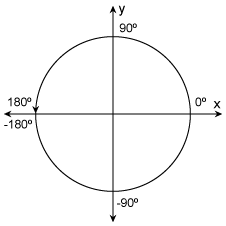
\includegraphics[width=0.4\textwidth]{figures/atan2d_graphic.png}
            \caption{Unit circle ranging from $-180^\circ$ to $180^\circ$, where the \textsc{x}-axis alligns with the East direction, and the \textsc{y}-axis alligns with North.}
            \label{fig:unitcircle}
        \end{SCfigure}
        
        \begin{equation}
        \label{eq:theta}
            \theta_{\mathbf{v}}(u, v) = 
            \begin{cases} 
                \text{tan}^{-1}\left(v/u\right)         & \text{if } u > 0 \\
                \text{tan}^{-1}\left(v/u\right)  + 180  & \text{if } v \geq 0 \; \wedge \; u < 0 \\
                \text{tan}^{-1}\left(v/u\right)  - 180  & \text{if } v < 0 \; \wedge \; u < 0 \\
                90                                              & \text{if } v > 0 \; \wedge \; u = 0 \\
                -90                                             & \text{if } v < 0 \; \wedge \; u = 0 \\
                \text{undefined}                                & \text{if } v = 0 \; \wedge \; u = 0
            \end{cases} 
        \end{equation}

        Knowing the angle of the wind vector $\theta_{\mathbf{v}}$, we can easily obtain the angle of the area vector $\theta_{\mathbf{A}}$ by rotating $\theta_{\mathbf{v}}$ by $90^\circ$ (Equation \ref{eq:thetaVtothetaA}). 

        \begin{equation}
        \label{eq:thetaVtothetaA}
            \theta_{\mathbf{A}}(\theta_{\mathbf{v}}) = \theta_{\mathbf{v}} + 90
        \end{equation}

        At this point, we have three pieces of information: the longitude $\lambda_P$ and latitude $\phi_P$ of the point at the centre of the grid cell, the size of the grid cell, and the fact that a line crosses the cell with an angle $\theta_{\mathbf{A}}$. If we can find the set of coordinates ($\left[\lambda_1,\, \phi_1\right]$, $\left[\lambda_2,\, \phi_2\right]$)  of the two points ($\mathbf{1}$, $\mathbf{2}$) that define this line, we can use the Haversine formula (Equation \ref{eq:haversine}), where $\Delta \phi = |\phi_1 - \phi_2|$, $\Delta \lambda = |\lambda_1 - \lambda_2|$ and $R$ is the radius of the earth $R = 6371$~km. The function $\mathbf{atan2}$ is defined as Equation \ref{eq:theta}.

        \begin{equation}
            \label{eq:haversine}
            \begin{aligned}
                a &= \text{sin}^2 (\Delta \phi / 2) + \text{cos}(\phi_1) \cdot \text{cos}(\phi_2) \cdot\text{sin}^2(\Delta \lambda /2) \\
                c &= \text{atan2}\left( \sqrt{a},\, \sqrt{1-a}\right) \\
                d &= R \cdot c
            \end{aligned}
        \end{equation}

        Given the conditions:
        
        \begin{equation}
            \begin{cases} 
                \text{TRUE} & (|\theta_{\mathbf{A}}| \leq 45) \vee \left(| \theta_{\mathbf{A}}| \geq 135 \right) \\
                \text{FALSE} & \text{else}
            \end{cases}
        \end{equation}
        
        We can define the transformations:
        
        \begin{equation} \label{eq:theta_transform}
            \theta' =
            \begin{cases} 
                90 - \left| \left(\theta_{\mathbf{A}} + 90\right) \bmod 360 - 180 \right| & \text{if } \text{TRUE} \\
                45 - \left| \left( \left|\theta_{\mathbf{A}}\right| + 90\right) \bmod 270 - 135 \right| & \text{else}
            \end{cases}
        \end{equation}
       
        Equation \ref{eq:theta_transform} defines transformations for $\theta' = f(\theta_{\mathbf{A}})$ such that the value of $\theta'$ is always between 0 and 45 as that is the range where $\text{tan}(\theta') \in (0,\, 1)$. The transformation functions ensure that when we calculate the coordinates for points $\mathbf{1}$ and $\mathbf{2}$  in Equations \ref{eq:lon1_transform} through \ref{eq:lat2_transform}, none fall outside the grid cell.
        
        \begin{equation} \label{eq:lon1_transform}
            \lambda_1 =
            \begin{cases} 
                \lambda_P + 0.05 \cdot
                    \begin{cases}
                        1  & \text{if } u \geq 0 \\
                        -1 & \text{else}
                    \end{cases}
                & \text{if } \text{TRUE} \\
                \lambda_P + 0.05 \cdot \tan(\theta') & \text{else}
            \end{cases}
        \end{equation}
        
        
        \begin{equation} \label{eq:lat1_transform}
            \phi_1 =
            \begin{cases} 
            \phi_P + 0.05 \cdot \tan(\theta') & \text{if } \text{TRUE} \\
            \phi_P + 0.05\cdot
                    \begin{cases}
                        1  & \text{if } v \geq 0 \\
                        -1 & \text{else}
                    \end{cases}
                & \text{else}
            \end{cases}
        \end{equation}
        
        
        \begin{equation} \label{eq:lon2_transform}
            \lambda_2 =
            \begin{cases} 
                \lambda_P - 0.05\cdot
                    \begin{cases}
                        1  & \text{if } u \geq 0 \\
                        -1 & \text{else}
                    \end{cases}
                    & \text{if } \text{TRUE} \\
                \lambda_P - 0.05 \cdot \tan(\theta') & \text{else}
            \end{cases}
        \end{equation}
        
        
        \begin{equation} \label{eq:lat2_transform}
            \phi_2 =
            \begin{cases} 
                \phi_P - 0.05 \cdot \tan(\theta') & \text{if } \text{TRUE} \\
                \phi_P - 0.05\cdot
                    \begin{cases}
                        1  & \text{if } v \geq 0 \\
                        -1 & \text{else}
                    \end{cases}
                    & \text{else}
            \end{cases}
        \end{equation}

        Following these steps and inserting the coordinates $\mathbf{1}\left[\lambda_1,\, \phi_1\right]$ and $\mathbf{2}\left[\lambda_2,\, \phi_2\right]$, into the Haversine set of equations given in Equation \ref{eq:haversine}, results in the length in metres of the cross-section vector area $\mathbf{A}$. This method makes the assumption that the Earth is perfectly spherical. The Earth's equitorial radius (6356~km) is 23~km larger than its polar radius (6378~km). This results in a maximum error of 0.5\% and is considered negligible for the distances measured for this project.
        
    \subsection{Obtaining Wind Energy}

        The energy of the windstorm is defined as the sum of the energy of the points in the area of interest for the duration of the windstorm event. The area of interest is every point within the following list of countries that is also within the boundary $\phi \in (42^\circ \rightarrow 72^\circ$\textbf{N}) and $\lambda \in (-12^\circ \rightarrow 32^\circ$\textbf{E}):

        Austria, Belgium, Czechia, Denmark, Estonia, Finland, France, Germany, Hungary, Ireland, Latvia, Liechtenstein, Lithuania, Luxemburg, the Netherlands, Norway, Poland, Slovakia, Spain, Sweden, Switzerland, and the UK.

        As we only count the energy of winds at or above 15~m/s, we do not need to know the exact borders of the windstorm, as the winds outside its area are unlikely to surpass that speed. A points energy can be calculated using Equation \ref{eq:KE}, with wind speed $\mathbf{v} = \sqrt{u^2_{\mathbf{v}} + v^2_{\mathbf{v}}}$, and the duration $t$ for which the equation is solved is $t = 1\text{hr}=3600\text{s}$. By changing the size of the list of countries which are counted towards the total energy of a windstorm, we can obtain the energy experienced during a windstorm event in a particular region or even a single country. This is useful for studying the severity of windstorms in different parts of Europe and for identifying zones particularly vulnerable to severe winds.
        
    \subsection{Challenges and Inaccuracies}

        Although the accuracy of the method depends on the spatial and temporal resolution of the reanalysis data used to calculate windstorm energies, its primary limitation arises from the storm "finding" technique. Specifically, the method sometimes struggles to pinpoint the precise start and end times of a storm. For certain storms, the 36-hour window before being recognised on land is insufficient. This is especially the case when the storm's centre moves parallel to the coast, likely tracing the path of a meridional jet stream. Consequently, the storm can accumulate significant damage to the infrastructure before the algorithm acknowledges it as an event. An example of this behaviour is the Great Storm of 87. 
        
        Another source of inaccuracy is the inability of the algorithm to distinguish between windstorm events that are only 2 to 3 days apart. In such a scenario, these storms are likely to be joined into a singular event, which may create outliers in the final results.